\title{Probing the subsurface karst features using time-frequency decomposition}

\author{Yangkang Chen\footnotemark[1]}
\address{
\footnotemark[1]Previously: Bureau of Economic Geology \\
John A. and Katherine G. Jackson School of Geosciences \\
The University of Texas at Austin \\
University Station, Box X \\
Austin, TX 78713-8924 \\
chenyk2016@gmail.com,
Currently: National Center for Computational Sciences \\
Oak Ridge National Laboratory \\
One Bethel Valley Road, \\
Oak Ridge, TN 37831-6008 \\
cheny@ornl.gov }
%INT-2016-0030

\lefthead{Chen}
\righthead{Probing the karst}
\maketitle

\DeclareRobustCommand{\dlo}[1]{\ifthenelse{\boolean{@revd}}{}{}}
\DeclareRobustCommand{\wen}[1]{%
\ifthenelse{\boolean{@revd}}{\textcolor{black}{#1}}{#1}}


\begin{abstract}
The high-resolution mapping of karst features is of great importance to \old{the} hydrocarbon discovery and recovery in the resource exploration field. However, currently, there are few effective methods specifically tailored for such mission. The 3D seismic data can reveal the existence of karsts to some extent but cannot obtain a precise characterization. I propose an effective framework for accurately probing the subsurface karst features using a well-developed time-frequency decomposition algorithm. More specifically, I introduce a frequency interval analysis approach for obtaining the best karsts detection result using an optimal frequency interval. A high resolution time-frequency transform is preferred in the proposed framework to capture the inherent frequency components hidden behind the amplitude map. Although the single frequency slice cannot provide a reliable karst depiction result, the summation over the selected frequency interval can obtain a high-resolution and high-fidelity delineation of subsurface karsts. I use a publicly available 3D field seismic dataset as an example to show the performance of the proposed method.  
\end{abstract}

%\begin{keywords}
%karst, time-frequency decomposition, synchrosqueezing wavelet transform
%\end{keywords}

\section{Introduction} 
Karst is a type of solutional caves that are usually formed in \old{the} soluble rock limestone when an aggressive fluid dissolves the rock. Subsurface karsting can produce a range of different structures, such as widened fissures and different types of cavities at all scales.  These may locally be partly or completely filled by
speleothems, sediments deposited by streams or breccia derived from stoping or collapse of the cave roof and walls \wen{\cite[]{karstthesis}}. \new{Commonly known karst features are fluid-enhanced faults \cite[]{su2005}, eroded caves, and sinkholes.} %incised valleys
The karst features are usually related with big petroleum reservoirs \wen{\cite[]{karstford}}. Understanding the spatial distribution of the karsts is of great importance to the discovery of hydrocarbons and their optimal recovery from these reservoirs. However, this can be very difficult \old{because of}\new{due to} several reasons. One reason is that the karsts are not uniformly distributed and exhibit an extreme spatial variability. Another reason is that the karst features are usually below seismic resolution\new{,} which makes them difficult to map. In this paper, I propose a high-resolution characterization approach for mapping the karst features by utilizing time-frequency decomposition of 3D seismic data.
 
Time-frequency decomposition offers extra information when analyzing seismic data, which has been extensively used in seismic data processing and interpretation \cite[]{jiajun2013,reine2009,rodriguez2012,fomel20132,tfpeak2015,yangkang2015sswt,liuwei20162,zhangdong20162}.
One of the most commonly used applications of time-frequency analysis is that deeper channels are usually \wen{of} stronger \wen{amplitude} at lower frequency in the time-frequency map\new{,} and the shallower flank of the channel has \dlo{stronger}\wen{larger} amplitude\dlo{s} at higher frequencies \wen{in the time-frequency map} \wen{\cite[]{liuwei2016,zixiang2016eage,liuwei2016eage}}. In addition, \dlo{TF}\wen{time-frequency} analysis can be used in estimating attenuation, pore-pressure prediction, detecting seismic unconformities, and some implementation of seismic chronostratigraphy \wen{\cite[]{tengfei2013}}. \wen{Over the past decades, time-frequency decomposition has found a panoply of applications in seismic data processing and interpretation \cite[]{jianlei2007}. Most time-frequency decomposition approaches are used in detecting low-frequency shadow \cite[]{castagna2003}, detecting paleochannels \cite[]{guochang20112}, reservoir characterization \cite[]{guoyin2015}, structural and stratigraphic delineation \cite[]{liuwei2016,yangkang2016eage}, arrivals picking of P or S wave modes \cite[]{pinnegar2003}.} In this paper, I  propose \dlo{a novel}\wen{an} application of the time-frequency decomposition in probing the subsurface karst features.  \dlo{Two}\wen{Four} \dlo{different} approaches with different analyzing resolutions are compared to offer more practical guidelines for utilizing the proposed approach. 

 Some researchers have mentioned the application of time-frequency decomposition approaches in delineating the subsurface karst feature, but most applications are not introduced in detail\old{s} \cite[]{satinder2007,gaynor2010}. The karst features are depicted based on the criteria that they are discontinuous in spatial domain and show frequency anomalies. The challenge in delineating karst feature lays in the fact that high-resolution delineation may result \new{in} many spurious frequency anomalies while low-resolution delineation may fail to depicted such valuable details. A method that can offer us freedom to control the characterization resolution and fidelity is \old{ strongly demanded}\new{in strong demand}. 

\section{Method}
Time-frequency decomposition maps a 1-D signal in the time domain into a 2-D image in time-frequency space, which can describe the local time-frequency variations
of geophysical properties. There have \dlo{existed}\wen{been} many different approaches for such decomposition mission, such as the continuous wavelet transform \wen{\cite[]{daubechies1992}}, S transform \wen{\cite[]{stockwell1996}}, and synchrosqueezing wavelet transform \wen{\cite[]{daubechies2011}}. I will not promote a new algorithmic advance here for better time-frequency decomposition, but instead, I will propose a novel and effective way for mapping the subsurface karst features based \new{on} a simple frequency interval analysis approach using 3D seismic data recorded at the surface of the targeted area. 

The algorithm can be summarized in three simple steps:  
\begin{itemize}
\item Step 1: Input the 3D seismic data, and define the minimum and maximum analyzing frequency $\omega_{\min}$ and $ \omega_{\max}$ and frequency interval distance $\Delta \omega$.
\item Step 2: Apply time-frequency decomposition to each trace of the 3D seismic data and sum the frequency components in each frequency interval $<\omega_i,\omega_{i}+\Delta \omega>$, $i=1,2,\cdots,N$, where $N$ denotes the number of frequency intervals, then reform the summed frequency components of different intervals into several 3D cubes that correspond to different frequency intervals.
\item Step 3: Output the different frequency cubes and analyze the results to pick the best frequency interval that can best depicts the karst features.
\end{itemize}

$\omega_{\min}$ and $\omega_{\max}$ are chosen based on the bandwidth of seismic data. A reference value can be $\omega_{\min}=1$Hz and $\omega_{\max}=100$Hz. The $\Delta \omega$ is the only parameter that may need several trials. One can test the $\Delta \omega$ from 5Hz to 30 Hz, and updating $\Delta \omega$ every 5Hz. The choice of $\Delta \omega$ is a compromise between analysis complexity and the characterization resolution.

It is worth mentioning that time-frequency based karst delineation approach is not new in geophysical study. A typical and standard way to extract subsurface karst features based on time-frequency decomposition is to extract different constant frequency slices, and then to select a certain frequency slice to best represent the karst features based on a prior knowledge and good correlation between the frequency slice and the amplitude map. However, the single frequency slice depiction is sometimes not  reliable since higher frequency may provide fine-scale delineation with higher resolution\new{,} while lower-frequency may provide large-scale result with lower resolution. The result of the contradiction in traditional approaches is that there might be spurious bright spots or unclear karsts representation. I will just mention the problem here and will show it in detail in the data example. The frequency interval analysis approach provides us a convenient way to control the resolution and reliability of finally depicted karsts by simply adjusting the frequency interval. Although determining the frequency interval still requires some efforts in its current version, \old{the}\new{my} experience shows that frequency interval is usually chosen as 5, 10, or 20Hz\old{, which is still not too many options to choose}.

\section{Study Area and Dataset}
The studied dataset is a 3D dataset that was a significant part of the total data base amassed during a two-year study of the Bend Conglomerate reservoir system in Boonsville Field in north-central Texas. The 3D Boonsville field dataset \wen{\cite[]{hardage1996,hardage1996b}} was made publicly available for educational training purposes for a broad range of industry and academic interests since 1996 by Bob Hardage from the Bureau of economic Geology at The University of Texas at Austin. A special property of this dataset is that it shows interesting karst phenomenon of deep Ellenburger carbonates, which generate collapse structures that have compartmentalized clastic Bend Conglomerate reservoirs 620 to 760 meters above the depths where collapse structures originate. The demonstration of the study area is shown in Figure \ref{fig:boons}. \wen{Figure \ref{fig:barnett-strat} shows the strati-graphic column of the Fort Worth Basin \cite[]{Pollastro07}. The formation of \old{interset}\new{interest} is the Ordovician-age Ellenburger carbonate section. The Ellenburger carbonate section creates near-vertical chimneys-like karst collapses. } The 3D seismic dataset is shown in Figure \ref{fig:old3d} and a selected 2D profile (crossline=75) is shown in Figure \ref{fig:old}. \dlo{If one looks carefully at Figure \ref{fig:old}, one can see some karst collapses around the depth of 1.75s, but the phenomenon is not very clear.} \wen{It can be observed that around the depth of 1.25s, there are some karst collapses, which is however, not very clear. In the next section, I will show a much better delineation result using time-frequency decomposition.  }

\AtEndDocument{
\begin{figure}[htb!]
  \centering
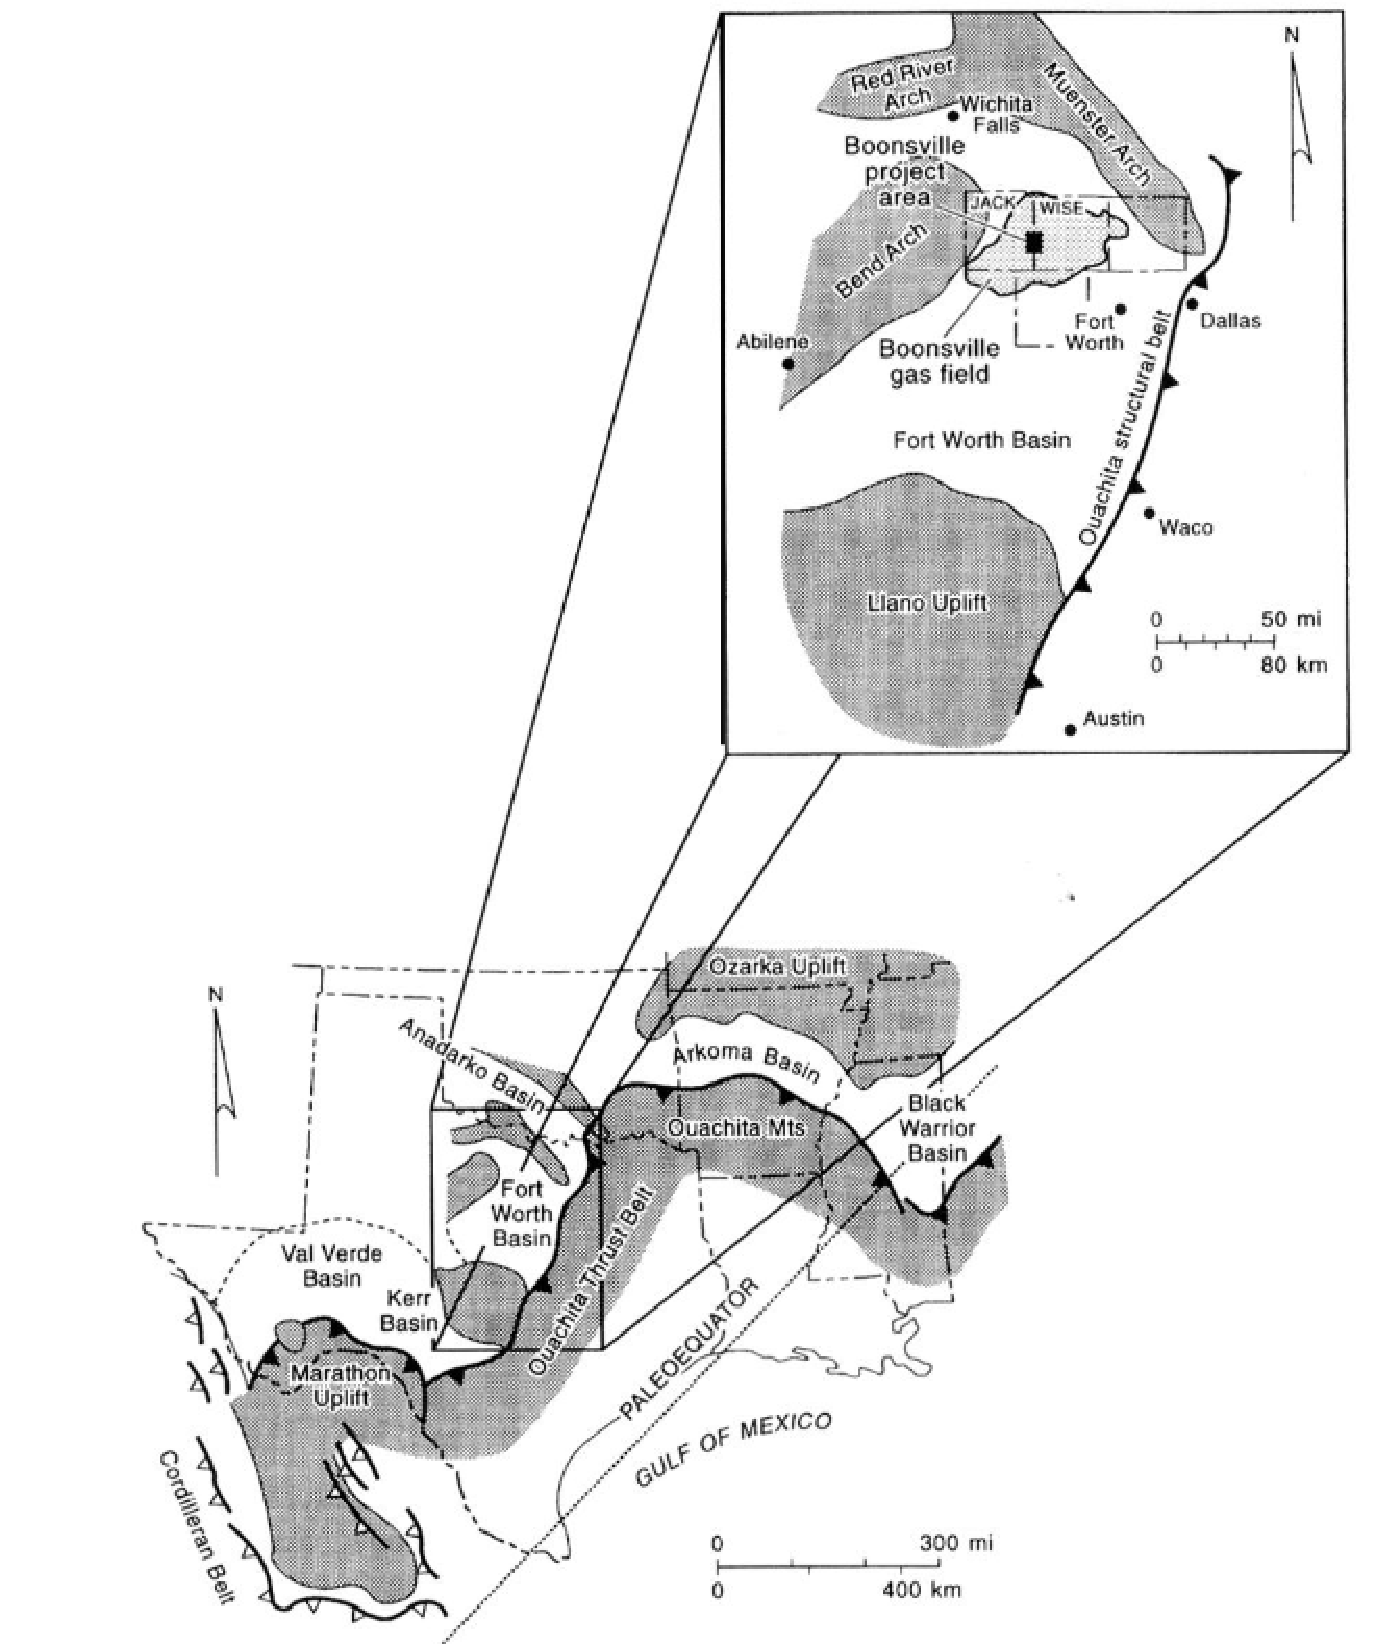
\includegraphics[width=\columnwidth]{Fig/boons}
   \caption{Middle Pennsylvanian paleogeographic map showing the Fort Worth Basin and other basins related to the Ouachita orogony and the
Boonsville project area. The solid rectangle on the Wise-Jack county line designates the site of the 3-D seismic survey, curtersy of \cite{hardage1996}.}
   \label{fig:boons}
\end{figure}

\begin{figure}[htb!]
  \centering
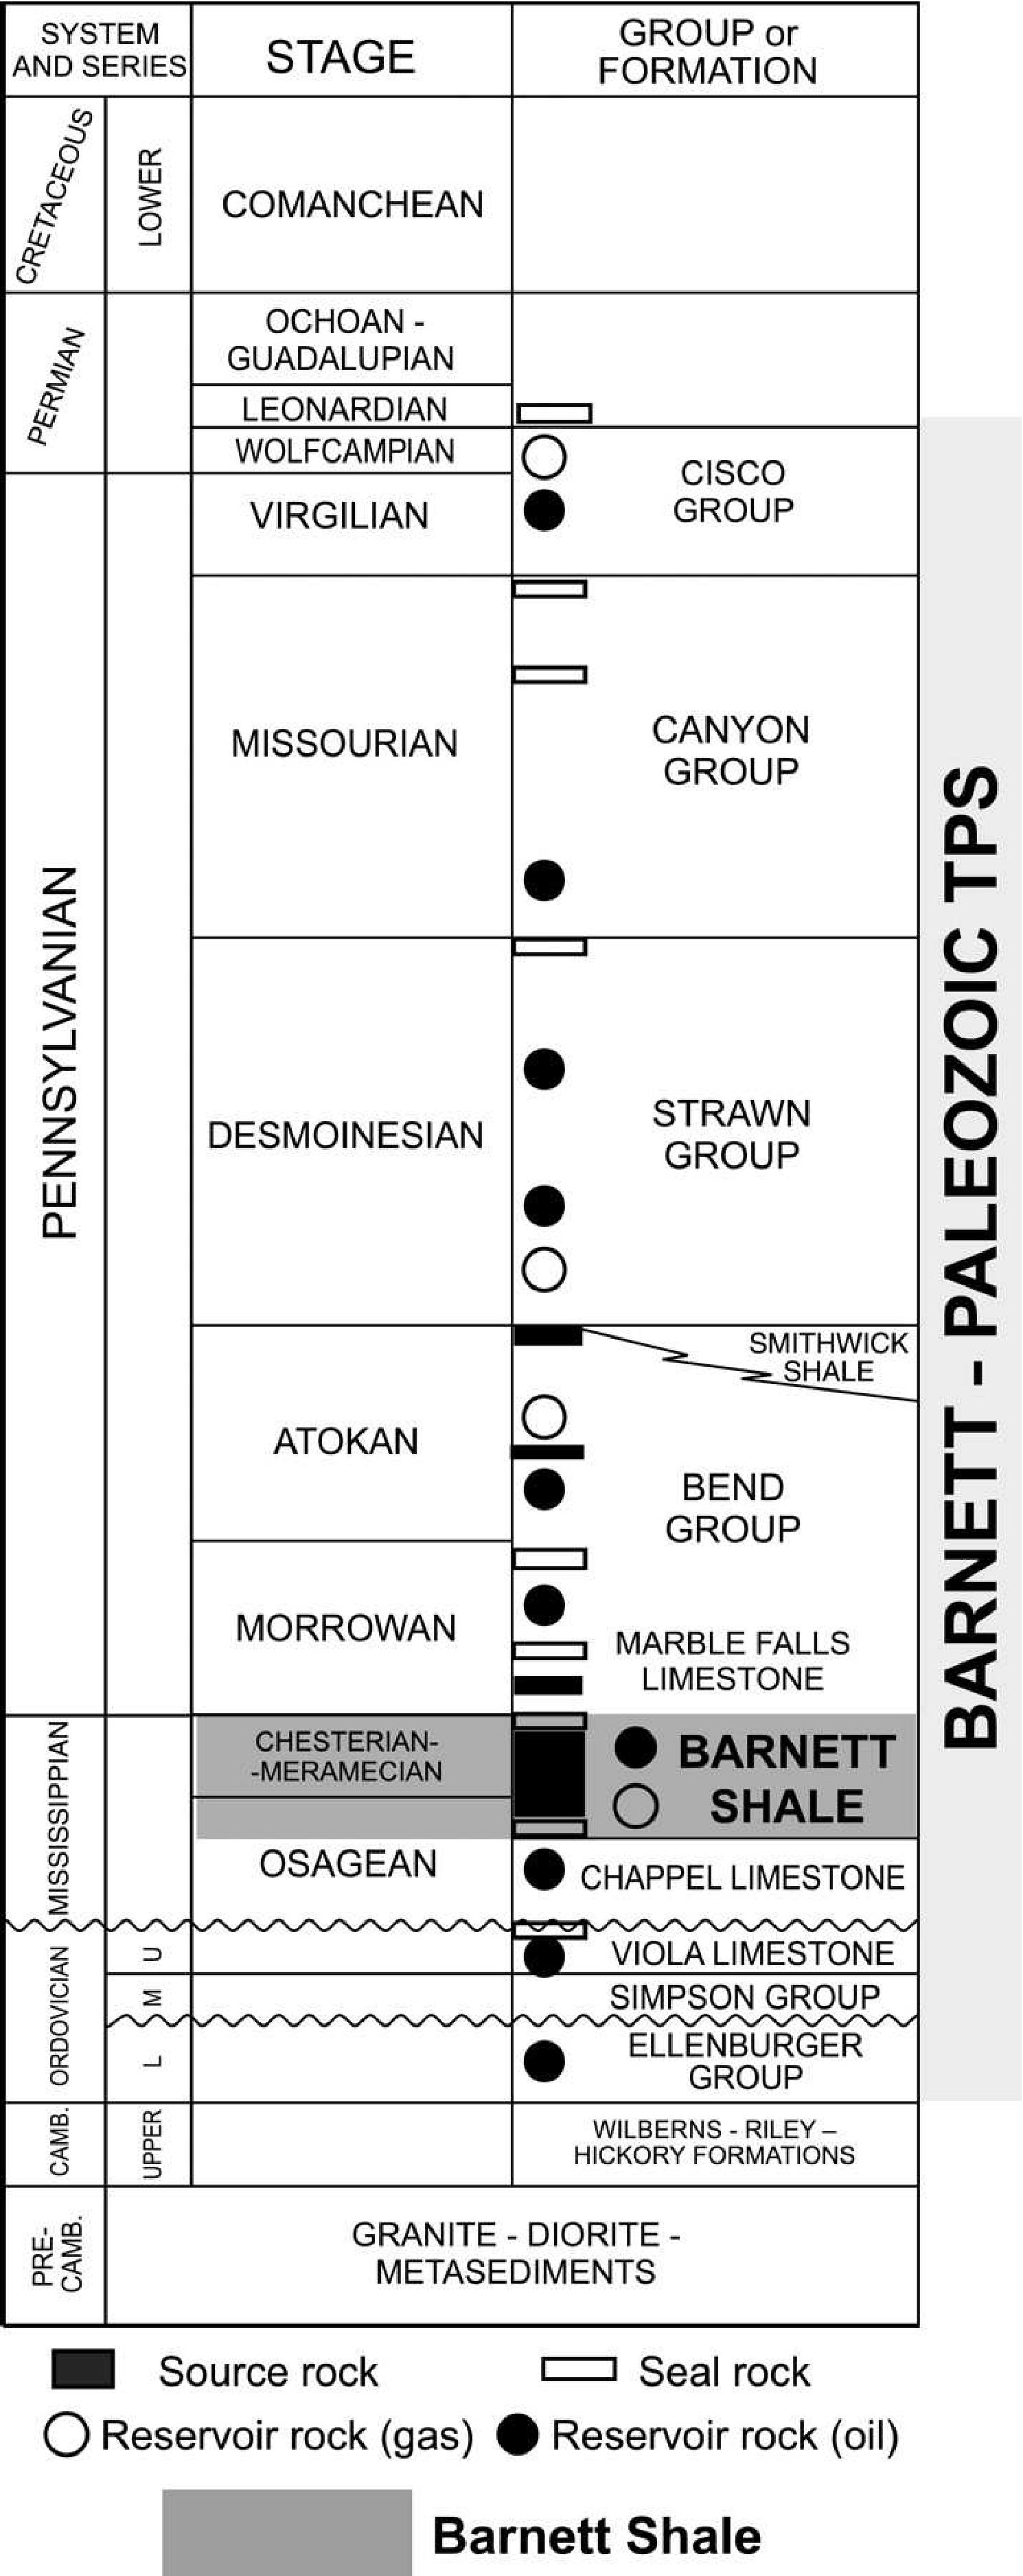
\includegraphics[width=0.45\columnwidth]{Fig/barnett-strat}
   \caption{\wen{Strati-graphic column of the Fort Worth Basin, curtersy of \cite{Pollastro07}. The target horizon is the deep Ordovician-age Ellenburger carbonate section which causes numerous karst collapses and significant disruptions in the overlaying strata.}}
   \label{fig:barnett-strat}
\end{figure}


\begin{figure}[htb!]
  \centering
\includegraphics[width=0.6\columnwidth]{boonsville_mac/Fig/old3d}
   \caption{3D \dlo{time-migrated} Boonsville dataset \wen{after time migration}.}
   \label{fig:old3d}
\end{figure}

\begin{figure}[htb!]
  \centering
    \subfigure[]{\includegraphics[width=0.45\columnwidth]{boonsville_mac/Fig/tfsswt1-2d3d-0}
   \label{fig:tfsswt1-2d3d-0}}
    \subfigure[]{\includegraphics[width=0.45\columnwidth]{boonsville_mac/Fig/tfsswt2-2d3d-0}
   \label{fig:tfsswt2-2d3d-0}}\\
    \subfigure[]{\includegraphics[width=0.45\columnwidth]{boonsville_mac/Fig/tfsswt3-2d3d-0}
   \label{fig:tfsswt3-2d3d-0}}
    \subfigure[]{\includegraphics[width=0.45\columnwidth]{boonsville_mac/Fig/tfsswt4-2d3d-0}
   \label{fig:tfsswt4-2d3d-0}}\\         
   \caption{3D karst features delineation result using SSWT with different frequency intervals. }
   \label{fig:tfsswt2-2d3d-0}
\end{figure}

\begin{figure}[htb!]
  \centering
  \subfigure[]{\includegraphics[width=0.5\columnwidth]{boonsville_mac/Fig/old}
   \label{fig:old}}\\
  \subfigure[]{\includegraphics[width=0.48\columnwidth]{boonsville_mac/Fig/lowf-st}
    \label{fig:lowf-st}}
  \subfigure[]{\includegraphics[width=0.48\columnwidth]{boonsville_mac/Fig/lowf-tfsswt2}
    \label{fig:lowf-tfsswt2}}
  \subfigure[]{\includegraphics[width=0.48\columnwidth]{boonsville_mac/Fig/lowf-stft}
    \label{fig:lowf-stft}}
  \subfigure[]{\includegraphics[width=0.48\columnwidth]{boonsville_mac/Fig/lowf-ltft}
    \label{fig:lowf-ltft}}        
   \caption{\wen{2D seismic section (crossline=75) and its karst mapping results. (a) Amplitude section. (b) Low frequency slice of ST. (c) Low frequency slice of SSWT. (d) Low frequency slice of STFT. (e) Low frequency slice of LTFT.}}
   \label{fig:lowf-st,lowf-tfsswt2}
\end{figure}

\begin{figure}[htb!]
  \centering
  \subfigure[]{\includegraphics[width=0.5\columnwidth]{boonsville_mac/Fig/old-z}
   \label{fig:old-z}}\\
  \subfigure[]{\includegraphics[width=0.48\columnwidth]{boonsville_mac/Fig/lowf-st-z}
    \label{fig:lowf-st-z}}
  \subfigure[]{\includegraphics[width=0.48\columnwidth]{boonsville_mac/Fig/lowf-sswt-z}
    \label{fig:lowf-sswt-z}}
  \subfigure[]{\includegraphics[width=0.48\columnwidth]{boonsville_mac/Fig/lowf-stft-z}
    \label{fig:lowf-stft-z}}
  \subfigure[]{\includegraphics[width=0.48\columnwidth]{boonsville_mac/Fig/lowf-ltft-z}
    \label{fig:lowf-ltft-z}}        
   \caption{\wen{Zoomed 2D seismic section (crossline=75) and its zoomed karst mapping results. (a) Amplitude section. (b) Low frequency slice of ST. (c) Low frequency slice of SSWT. (d) Low frequency slice of STFT. (e) Low frequency slice of LTFT.}}
   \label{fig:lowf-st-z,lowf-sswt-z}
\end{figure}

\begin{figure}[htb!]
  \centering
    \subfigure[]{\includegraphics[width=0.4\columnwidth]{boonsville_mac/Fig/tf-s}
   \label{fig:tf-s}}
    \subfigure[]{\includegraphics[width=0.4\columnwidth]{boonsville_mac/Fig/tf-ss}
   \label{fig:tf-ss}}\\    
    \subfigure[]{\includegraphics[width=0.4\columnwidth]{boonsville_mac/Fig/tf-stft}
   \label{fig:tf-stft}}
    \subfigure[]{\includegraphics[width=0.4\columnwidth]{boonsville_mac/Fig/tf-ltft}
   \label{fig:tf-ltft}}\\      
   \caption{\wen{Time-frequency maps of the 80th trace in the 2D seismic section as shown in Figure \ref{fig:old}, using (a) ST and using (b) SSWT. (c) STFT. (d) LTFT. The selected trace is highlighted by the blue line in Figure \ref{fig:old}.}}
   \label{fig:tf-s,tf-ss,tf-stft,tf-ltft}
\end{figure}



\begin{figure}[htb!]
  \centering
  \subfigure[]{\includegraphics[width=0.21\columnwidth]{boonsville_mac/Fig/sswt-0}
   \label{fig:sswt-0}}  
  \subfigure[]{\includegraphics[width=0.21\columnwidth]{boonsville_mac/Fig/sswt-1}
   \label{fig:sswt-1}}
  \subfigure[]{\includegraphics[width=0.21\columnwidth]{boonsville_mac/Fig/sswt-2}
    \label{fig:sswt-2}}
  \subfigure[]{\includegraphics[width=0.21\columnwidth]{boonsville_mac/Fig/sswt-3}
    \label{fig:sswt-3}}
  \subfigure[]{\includegraphics[width=0.21\columnwidth]{boonsville_mac/Fig/sswt-4}
    \label{fig:sswt-4}} 
  \subfigure[]{\includegraphics[width=0.21\columnwidth]{boonsville_mac/Fig/sswt-5}
   \label{fig:sswt-5}}
  \subfigure[]{\includegraphics[width=0.21\columnwidth]{boonsville_mac/Fig/sswt-6}
    \label{fig:sswt-6}}
  \subfigure[]{\includegraphics[width=0.21\columnwidth]{boonsville_mac/Fig/sswt-7}
    \label{fig:sswt-7}}
  \subfigure[]{\includegraphics[width=0.21\columnwidth]{boonsville_mac/Fig/sswt-8}
    \label{fig:sswt-8}}  
  \subfigure[]{\includegraphics[width=0.21\columnwidth]{boonsville_mac/Fig/sswt-9}
   \label{fig:sswt-9}}
  \subfigure[]{\includegraphics[width=0.21\columnwidth]{boonsville_mac/Fig/sswt-10}
    \label{fig:sswt-10}}
  \subfigure[]{\includegraphics[width=0.21\columnwidth]{boonsville_mac/Fig/sswt-11}
    \label{fig:sswt-11}}
  \subfigure[]{\includegraphics[width=0.21\columnwidth]{boonsville_mac/Fig/sswt-12}
    \label{fig:sswt-12}}      
  \subfigure[]{\includegraphics[width=0.21\columnwidth]{boonsville_mac/Fig/sswt-13}
    \label{fig:sswt-13}}
  \subfigure[]{\includegraphics[width=0.21\columnwidth]{boonsville_mac/Fig/sswt-14}
    \label{fig:sswt-14}}
  \subfigure[]{\includegraphics[width=0.21\columnwidth]{boonsville_mac/Fig/sswt-15}
    \label{fig:sswt-15}}             
   \caption{\wen{Constant frequency slices using SSWT. The frequency range is from 21 to 81 Hz. Frequency interval is 4 Hz. }}
   \label{fig:sswts}
\end{figure}

}


Some structure-related anomalies, such as the faults, discontinuities, karst collapses, are not always easily viewed from the original amplitude-based seismic profile. There \old{have existed}\new{are} many approaches in the literature \old{for better viewing}\new{which better highlights} the structural anomalies. One of the most \old{used}\new{common} methods is to define \new{a} new seismic attribute which is sensitive to the structural anomalies\old{ to show clear delineation of the structural anomalies} \cite[]{wenkai2015,xieqian2015eage2}. The 3D dataset from the Boonsville field contains typical karst phenomenon, as shown in Figures \ref{fig:old3d} and \ref{fig:old}. But\new{,} from the original seismic reflections, the phenomenon is not obvious. 

\section{Results}
By utilizing the proposed frequency interval analysis method, one can divide the total frequency \old{band}\new{range} into different sub-bands\new{,} and analyze the structural behaviors delineated from the sub-bands. In this paper, \wen{I use the synchrosqueezing wavelet transform (SSWT) \cite[]{daubechies2011,yangkang2014sswt,xieqian2015eage} for the time-frequency delineation of the karsts. } \dlo{I define the}\wen{I let} $\omega_{\min}=1$\new{Hz}, $\omega_{\max}=80$\new{Hz}, and $\Delta \omega=20$\new{Hz}, which \dlo{are}\wen{is} the optimal parameter combination for this dataset. \new{I choose $\omega_{\min}=1$ Hz and $\omega_{\max}=80$ Hz by looking at the averaged frequency spectrum of the seismic data and finding out that amplitude spectrum beyond 80 Hz or below 1 Hz is almost negligible. $\Delta \omega=20$\new{Hz} is decided by comparing the delineation results (as shown in Figure \ref{fig:tfsswt2-2d3d-0}) with $\Delta \omega=5,10,20$ Hz, respectively, and founding out that $\Delta \omega=20$Hz gives the best performance. }  The four 3D cubes that correspond to four different frequency intervals ($<1,20>$ Hz, $<21,40>$ Hz, $<41,60>$ Hz, and $<61,80>$ Hz) are shown in Figures \ref{fig:tfsswt1-2d3d-0} to \ref{fig:tfsswt4-2d3d-0}, respectively. \dlo{Please focus}\wen{Focusing} on the target layer from 1.0 s to 1.4 s, it is obvious that the result of the frequency interval $<21,40>$ clearly shows the distribution of the karsts. Please note that the closer the color is to blue, the higher possibility that area is karst. \new{The collapsed karsts are not formed during continuous sedimentation and thus is usually composed of complicated components. There are no layered structures inside the karsts, which will make seismic wave go through a strong scattering process when traveling through the karst media. The strong scattering will be revealed in seismic image as discontinuities, which will be further revealed in time-frequency maps as low amplitude phenomenon in the dominant frequency range. Thus, the blue (close to zero) is of higher likehood of karst.} I then select the best 3D karst characterization result of the frequency interval $<21,40>$ Hz and show it in detail in Figure \ref{fig:tfsswt2-2d3d,tfsswt2-2d3d-2,tfsswt2-2d3d-3,tfsswt2-2d3d-4} and will discuss about the details later.  

\AtEndDocument{
\begin{figure*}[ht!]
  \centering
  \subfigure[]{\includegraphics[width=0.44\columnwidth]{boonsville_mac/Fig/tfsswt2-2d3d}
    \label{fig:tfsswt2-2d3d}}
  \subfigure[]{\includegraphics[width=0.44\columnwidth]{boonsville_mac/Fig/tfsswt2-2d3d-2}
    \label{fig:tfsswt2-2d3d-2}}
  \subfigure[]{\includegraphics[width=0.45\columnwidth]{boonsville_mac/Fig/tfsswt2-2d3d-3}
    \label{fig:tfsswt2-2d3d-3}}
  \subfigure[]{\includegraphics[width=0.45\columnwidth]{boonsville_mac/Fig/tfsswt2-2d3d-4}
    \label{fig:tfsswt2-2d3d-4}}
   \caption{3D karst features mapping results (flat view) using SSWT with different time (top), crossline (left) and inline (right) slices. (a) Crossline=75, inline=80, time=1.2s. (b) Crossline=45, inline=80, time=1.2s. (c) Crossline=75, inline=50, time=1.2s. (d) Crossline=75, inline=80, time=1.1s.}
   \label{fig:tfsswt2-2d3d,tfsswt2-2d3d-2,tfsswt2-2d3d-3,tfsswt2-2d3d-4}
\end{figure*}


\begin{figure}[htb!]
  \centering
  \subfigure[]{\includegraphics[width=0.8\columnwidth]{strata/Fig/stra-int}
    \label{fig:stra-int}}
  \subfigure[]{\includegraphics[width=0.8\columnwidth]{strata/Fig/stra-tf}
    \label{fig:stra-tf}}
  
   \caption{\wen{(a) 3D amplitude section with picked horizons overlaid. %(b) 3D absolute value amplitude section. 
   (b) Time-frequency delineation result with picked horizons overlaid. Top pink line denotes Caddo strata. Middle green line denotes the Vineyard strata. Bottom blue line denotes the Ellenburger strata.} }
   \label{fig:stra-int,stra-tf}
\end{figure}

\begin{figure}[htb!]
  \centering
  \subfigure[]{\includegraphics[width=0.45\columnwidth]{strata/Fig/stra1}
    \label{fig:stra1}}
  \subfigure[]{\includegraphics[width=0.45\columnwidth]{strata/Fig/stra2}
    \label{fig:stra2}}
   \subfigure[]{\includegraphics[width=0.45\columnwidth]{strata/Fig/stra3}
    \label{fig:stra3}}
  \subfigure[]{\includegraphics[width=0.45\columnwidth]{strata/Fig/stra4}
    \label{fig:stra4}} 
   \caption{\wen{Different strata slices from the time-frequency delineation result, shown in Figure \ref{fig:stra-tf}. (a) Top of Caddo. (b) Strata slice between Caddo and Vineyard. (c) Top of Vineyard. (d) Strata slice between Vineyard and the base.} }
   \label{fig:stra1,stra2,stra3,stra4}
\end{figure}

}


I then take the selected 2D section for further analysis. I compare the performance using \dlo{two}\wen{four} different time-frequency decomposition approaches: \wen{the} S transform\dlo{ and }\wen{, the} SSWT transform\wen{, the short time Fourier transform (STFT), and the local attribute based time-frequency transform (LTFT) \cite[]{guochang20113} }.  The delineation results using \dlo{ST and SSWT}\wen{ST, SSWT, STFT, and LTFT} are shown in Figures \dlo{\ref{fig:lowf-st} and \ref{fig:lowf-tfsswt2}}\wen{\ref{fig:lowf-st}, \ref{fig:lowf-tfsswt2} , \ref{fig:lowf-stft} , and \ref{fig:lowf-ltft} }, respectively. The result from SSWT is very appealing because those karst collapses are all depicted by the time-frequency decomposition (see those \wen{pink} frame boxes)\new{,} and \old{those}\new{the} collapse areas are all corresponding to small amplitude in the low frequency slice. However, \dlo{ST}\wen{all other time-frequency transforms} cannot decompose the seismic data in such way.  In order to make the comparison clearer, I zoom a part from each figure in Figure \ref{fig:lowf-st,lowf-tfsswt2} and show them in Figure \ref{fig:lowf-st-z,lowf-sswt-z}. The zoomed area is highlighted by the black frame boxes in Figure \ref{fig:lowf-st,lowf-tfsswt2}. In Figure \ref{fig:lowf-st-z,lowf-sswt-z}, the blue color in Figure \ref{fig:lowf-sswt-z} correlates well with the collapsed area in Figure \ref{fig:old-z}. The best mapping of karsts using SSWT is due to its high resolution property when analyzing 1D non-stationary seismic signals. Figure \ref{fig:tf-s,tf-ss,tf-stft,tf-ltft} shows time-frequency decomposition results of the 80th trace of the 2D seismic section as shown in Figure \ref{fig:old}\new{,} using four different approaches (ST, SSWT, STFT, and LTFT). The selected trace is highlighted by blue in Figure \ref{fig:old}.  From the comparison, one can see that SSWT has a much higher frequency resolution than ST, STFT, and LTFT. From the single-trace time-frequency slice one can judge roughly in which depth the data show abnormal frequency, and what their corresponding dominant frequency components are. In order to show superior performance of the frequency interval analysis approach as introduced in \old{the}\new{this} paper\new{,} over the traditional single frequency slice analysis approach, I plot 16 single frequency slices in Figure \ref{fig:sswts}. The frequency range is from 21 Hz to 81 Hz, and I plot the frequency slices every 4 Hz. It can be observed that the time-frequency decomposition results of subsurface properties are either of too low resolution\new{,} as shown in the low frequency slices, or of too high resolution as shown in high frequency slices. \old{The depicted results via constant single frequency slice do not correlate with the karst collapses and thus no frequency slice can be reliable to depicted the subsurface karst features.} 


Figure \ref{fig:tfsswt2-2d3d,tfsswt2-2d3d-2,tfsswt2-2d3d-3,tfsswt2-2d3d-4} shows 3D karst delineation results (flat view) using SSWT with different time (top), crossline (left) and inline (right) slices. Figure \ref{fig:tfsswt2-2d3d} differs from \ref{fig:tfsswt2-2d3d-2} by different crossline sections. From the comparison between Figures \ref{fig:tfsswt2-2d3d} and \ref{fig:tfsswt2-2d3d-2}, one can see clearly how the karst varies along the crossline direction: the karst becomes weaker from crossline 75 to crossline 50. In the same way, one can study the karst variation along the inline direction by comparing Figures \ref{fig:tfsswt2-2d3d} and \ref{fig:tfsswt2-2d3d-3}. %From the comparison between Figures \ref{fig:tfsswt2-2d3d} and \ref{fig:tfsswt2-2d3d-4}, one can conclude that the karstification becomes weaker from 1.2 s to 1.1 s. 
It is also possible to evaluate the volume of the karst controlled area by looping along different directions in the 3D volume (Figure \ref{fig:tfsswt2-2d3d-0}), which is closely related with the karst controlled reserve.  Figure \ref{fig:stra-int} shows an interpreted 3D seismic section with three key stratas highlighted. The top pink line, middle green line, and bottom blue line denote the Caddo strata,  the Vineyard strata, and the Ellenburger strata, respectively. Figure \ref{fig:stra-tf} shows the time-frequency delineation result of the karsts overlaid by the picked three horizons. The Upper Caddo is the top boundary of the productive Bend Conglomerate section, and the Upper Vineyard is a sequence near the base of the Bend Conglomerate section. The Bend Conglomerate section is of Middle Pennsylvanian age (also known as Atokan) and is targeted throughout the 1980s and 1990s as it contains several oil\&gas bearing reservoirs. \old{It has a}\new{The} thickness \new{is} around 300-360 meters in this area\new{,} with a depth from 1370 to 1830 meters \cite[]{hardage1996,hardage1996b}.   It can be observed from the karsts mapping result shown in Figure \ref{fig:stra-tf} that the karsts spreads a deep range from the Upper Caddo to the base of Ellenburger. %As the general karsts delineation result correlates very well with the amplitude section, blue color under the Ellenburger strata even indicates that the collapses start even earlier than the Ellenburger carbonate. 
I also selected different strata slices from Figure \ref{fig:stra-tf} and show them in Figure \ref{fig:stra1,stra2,stra3,stra4}. Figure \ref{fig:stra1} shows a structure surface of the top of Caddo. Figure \ref{fig:stra2} shows a structure surface between Caddo and Vineyard. Figure \ref{fig:stra3} shows a structure surface on the top of Vineyard. Figure \ref{fig:stra4} shows a structure surface between Vineyard and the base of Ellenburger carbonate section. It can be observed that from up to down, the main color turns from cool (blue) to warm (red), indicates that the karstification weakens as the depth increases, which is consistent with the fact that the consolidation becomes stronger as the depth increases and make the deeper strata has stronger collapses and less karsts.  
 
\new{The Boonsville 3D dataset consolidate the proposed frequency interval analysis method in delineating subsurface karst collapses. When I use the term \emph{karst collapses}, I intend to refer to all those commonly seen karst features, such as incised valleys, eroded caves, sinkholes, and so on. While the reasons causing these karst features are different, they will all cause more or less depressions or collapses to the overburden strata and have a similar situation as the one presented in the Boonsville example. There is a large potential that the proposed framework can be successfully used in any type of karst features, and future validation of the framework on more field datasets are worth being done. The sediment or mud-filled collapse features may not cause significant differences of anomalies in amplitude spectrum and they will both show irregularities on the 3D seismic images since seismic wave will experience strong scattering effects when traveling through the collapsed area. But future investigation should be done to validate this inference. } 
 
\section{Conclusion}
Accurate\old{ly} mapping \new{of}\old{the} karst features is crucial for the resources exploration and recovery. The 3D seismic data can offer some insights in the spatial distribution of the karsts\new{,} but with low resolution, since the boundary of karst caves cannot be clearly delineated and the small-scale kart features are smeared in the seismic reflections. I propose to use time-frequency decomposition via a frequency interval analysis approach to accurately map the subsurface karst features with high resolution and accuracy. The time-frequency resolution can affect the final depicted result\new{,} and I suggest\dlo{ to use} \wen{using} the high-resolution synchrosqueezing wavelet transform (SSWT) to perform such task. The frequency interval analysis approach can provide us with more freedom in controlling the resolution and reliability of the \old{finally}\new{final} depicted result\new{,} compared with the traditional single frequency slice based approach. The proposed method is easy to implement and \dlo{should be paid}\wen{deserves} more attention to assist in geological research on the topic of karst evolution.


\section{Acknowledgements}
I would like to thank Summer Li, Qian Xie, Shuwei Gan, Wei Liu, Zixiang Cheng, Tingting Liu for helpful discussions\new{,} and Bob Hardage for making the Boonsville dataset publicly available.  I also thank associate editor Hongliu Zeng, \new{Victor Aarre}, and two anonymous reviewers for constructive suggestions that improved the manuscript greatly\new{.}\old{ and}\new{ Finally, thanks to} Dmytro Iatsenko for sharing the SSWT code\old{s} online: 
\begin{verbatim}
http://www.physics.lancs.ac.uk/research/nbmphysics/diats/tfr/.
\end{verbatim}
\newpage

\listoffigures
\bibliographystyle{jge}
\bibliography{sswt}







